\chapter{The hydrogen atom}
\addtocontents{toc}{\contentsline{chapter}{The hydrogen atom}{\protect\pageref{annotation}}}
\label{ch:basics}

This chapter explains how the Schr\"odinger and Dirac equations can be solved for the hydrogen atom and define the angular and radial hydrogen wavefunctions, while highlighting differences between the relativistic and non-relativistic calculations.

\section{Hydrogen atom in the Schr\"odinger theory}
In non-relativistic quantum mechanics the Hamiltonian of a hydrogen-like atom is given by~\cite{LandauQM}:
\begin{equation}\label{SchH}
\widehat{H}=\widehat{H}^{\rm{kin}} + \widehat{V} = -\frac{1}{2}\nabla^2 - \frac{Z}{r},
\end{equation}
where $\nabla^2$ is the Laplace operator and $Z$ the nuclear charge. Expanding in spherical coordinates, we get:
\begin{equation}\label{SchSpher}
	\frac{1}{r^2}\partial_r(r^2 \partial_r \psi)+\frac{1}{r^2 \sin \theta}\partial_\theta(\sin \theta \partial_\theta \psi)+\frac{1}{r^2\sin^2 \theta} \partial_{\varphi}^2 \psi+2\left(\frac{Z}{r}+E\right)\psi = 0.
\end{equation}
This equation can be separated into the radial and angular parts, i.e. the wavefunction can be written as:
\begin{equation}
	\psi(r,\theta,\varphi) = R(r)Y(\theta,\varphi).
\end{equation}
This splits~\eqref{SchSpher} into separate radial and angular equations. The details of solving both of them are given in Appendix~\ref{app:hydrogen}, while here we simply present the conclusions.

The functions satisfying the angular equation are called spherical harmonics. They are the eigenvectors of the angular momentum operator $\widehat{L} = -i \vec{r} \times \vec{\nabla}$ squared and its projection on the $z$ axis~\cite{biedenharn1984angular}. They can be explicitly written, as:
\begin{equation}
	Y_l^m (\theta, \varphi)=N_{lm}P_l^m(\cos \theta)e^{i m \varphi},
\end{equation}
where $N_{lm}$ are appropriate normalization constants, and $P_l^m$ are associated Legendre polynomials (see Appendix~\ref{app:Legendre} for details). The quantum number $l$ represents the value of angular momentum and $m$ its projection on the $z$ axis (see figure~\ref{AngMomFig}). They are both integers, such that $|m|\leq l$. Spherical harmonics form an orthonormal basis of all scalar functions on the unit sphere so all angular functions can be expanded in spherical harmonics, not unlike the Fourier series expansion in sines and cosines on the unit circle.

For our purposes, their most important properties are:
\begin{equation}
	\text{1) orthonormality: } \int Y_l^{m*}(\Omega) Y_{l'}^{m'} (\Omega) d\Omega=\delta_{l,l'}\delta_{m,m'},
\end{equation}
where the solid angle $d\Omega = \sin \theta d\theta d\varphi$,
\begin{equation}
\text{2) conjugate reflection: } Y_l^{m*} = (-1)^m Y_l^{-m}.
\end{equation}
and the fact that values of integrals of three spherical harmonics are tabulated using the so-called 3-$j$ symbols~\cite{cowan1981theory}: 
  \begin{align} \label{3jInt}
\text{3)  }	\int Y_{l_{1}}^{m_{1}}(\Omega)& Y_{l_{2}}^{m_{2}}(\Omega)
	Y_{l_{3}}^{m_{3}}(\Omega) d\Omega \nonumber \\
	&=
	\sqrt{\frac{(2l_1+1)(2l_2+1)(2l_3+1)}{4 \pi}}
	\begin{pmatrix} l_1 & l_2 & l_3 \\ 0 & 0 & 0 \end{pmatrix}
	\begin{pmatrix}l_1 & l_2 & l_3\\ m_1 & m_2 & m_3 \end{pmatrix}.
\end{align}

\begin{figure} [t] 
	\centering
	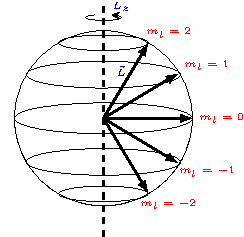
\includegraphics[width=69mm]{Graphs/AngularMomentum.pdf} 
	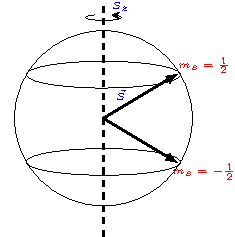
\includegraphics[width=69mm]{Graphs/Spin.pdf} 
	\caption{Visual representations of the angular momentum (left) and spin (right) quantum numbers. $m_l$ and $m_s$ represent projections on the z-axis of the angular momentum and spin respectively.} \label{AngMomFig}
\end{figure}

%\begin{figure} [t] 
%	\centering
%	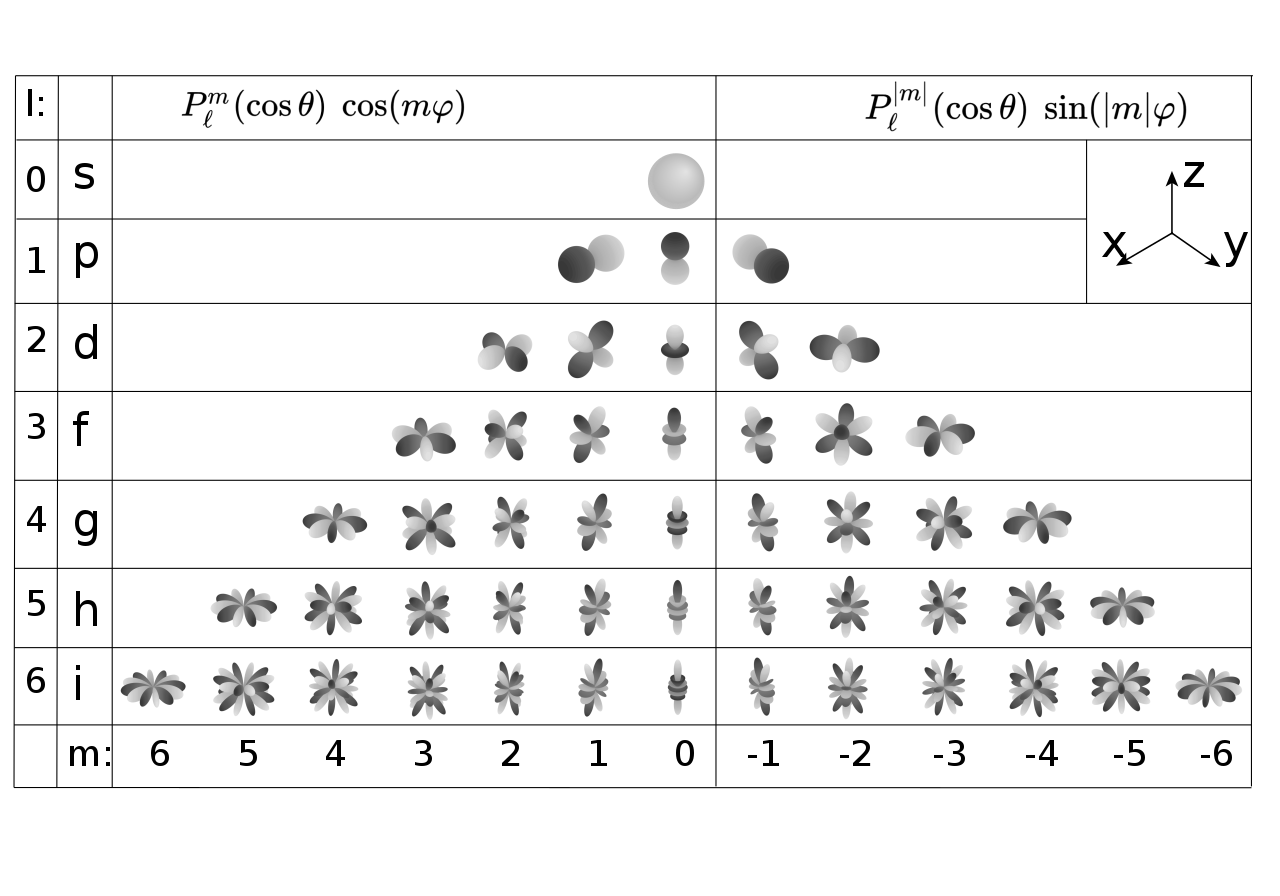
\includegraphics[width=119mm]{Graphs/SphericalHarmonicsStolen.png} 
%	\caption{Visual representations of the first few real spherical harmonics. %Graphic from the Wikipedia %article.
%	} \label{sphHarFig}
%\end{figure}

The functions satisfying the radial equation are in general expressed with Whittaker functions (see Appendix~\ref{app:Whittaker} for details). The bound states of the hydrogen-like atom, called hydrogen-like wavefunctions correspond to 
\begin{equation} \label{SchEnergy}
    E=\frac{-Z^2}{2n^2},
\end{equation} 
 where $n \in \mathbb{N}$ is the principal quantum number. The whittaker functions at such resonant energies reduce to a product of an exponential and a Laguerre polynomial~\cite{LandauQM}:
\begin{equation}
	R_{n,l,Z}(r)=N_{n,l}Z^{3/2}(Z r)^l L_{n-l-1}^{2l+1}\left(\frac{2Z}{n}r \right),
\end{equation}
where $N_{nl}$ is a normalization constant ensuring that the radial wavefunctions are orthonormal with respect to the principal quantum number:
\begin{equation}
	\int R_{n,l,Z}(r) R_{k,l,Z}(r) r^2 dr = \delta_{n,k}.
\end{equation}
Orthonormality is not preserved if the values of $Z$ are different.

Explicitly, Laguerre polynomials are given, by~\cite{AS}:
\begin{equation} \label{Laguerre}
    L_n^\alpha (x) = \sum_{i=0}^n \frac{(\alpha+i)!}{(n-i)!(i+\alpha)!}\frac{(-x)^i}{i!}.
\end{equation}

Finally, to account for the spin degree of freedom, a separate orthonormal wavefunction $\chi$ is introduced, indexed by the spin quantum number $s$, with two possible values $s=\uparrow \downarrow $. The total hydrogen-like wavefunction in Schr\"odinger theory is then given by:
\begin{equation}
	\psi_{n,l,m,s,Z}(r,\theta,\varphi) = R_{n,l,Z}(r)Y_{l,m}(\theta,\varphi)\chi_s.
\end{equation}

It is a well-established convention to refer to electronic states characterized by hydrogen-like quantum numbers, using a letter from the set $\{s,p,d,f\}$\footnote{For purely historical reasons these letters are abbreviations of "sharp", "principal", "diffuse" and "fundamental", which refer to the appearance of their observed fine structure~\cite{ebbing2007general}.} to denote the angular momentum quantum number $l$ while keeping the numerical values of the quantum numbers $n$ and $m$. For example $2p_{-1}$ refers to a state characterized by $n=2$, $l=1$, and $m=-1$.

\begin{figure} [t] 
	\centering
	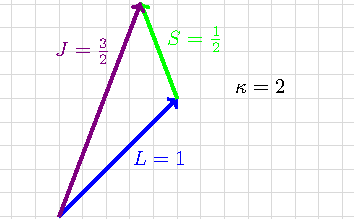
\includegraphics[width=69mm]{Graphs/AngularMomentum2.pdf} 
	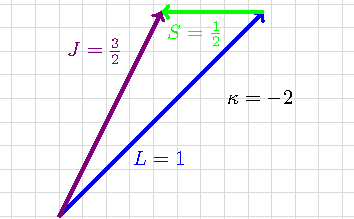
\includegraphics[width=69mm]{Graphs/AngularMomentum1.pdf} 
	\caption{Visual representation of the coupling of angular momentum $\vec{L}$ and spin $\vec{S}$ into the total angular momentum $\vec{J}$. Lengths of the corresponding vectors are given by $\sqrt{l(l+1)}$, $\sqrt{s(s+1)}$, and $\sqrt{j(j+1)}$ respectively. Different signs of the relativistic angular quantum number $\kappa$ represent different combinations of $l$ and $s$ into the same value of $j$.} \label{TotalAngMomFig}
\end{figure}

\section{Hydrogen atom in the Dirac theory}
\label{sec:Dirachydro}

In 1928 Paul Dirac proposed a relativistic equivalent of the Schr\"odinger Hamiltonian:
\begin{equation}
 	\widehat{H} = \vec{\alpha} \cdot \vec{\nabla} + \alpha_0 c,
 \end{equation}
where the four quantities $\{\alpha_0,\alpha_1,\alpha_2,\alpha_3\}$ are required to satisfy the anticommutation relations:
\begin{equation} \label{alphaCondition}
\alpha_{\mu} \alpha_{\nu}+\alpha_{\nu} \alpha_{\mu} =2\delta_{\mu \nu}.
\end{equation}
This condition cannot be satisfied by any set of complex numbers, so these quantities must be more complicated objects. In fact their smallest possible representation uses $4\times4$ matrices. The most commonly used one is:
\begin{equation} \label{DiracAlpha}
    \alpha_i = \left(\begin{matrix}0 & \sigma^i\\ \sigma^i & 0 \end{matrix}\right),~~~~~~~~~~\alpha_0 = \left(\begin{matrix} I & 0 \\ 0 & -I \end{matrix}\right).
\end{equation}
where $I$ is the identity matrix and $\sigma$ denote the Pauli matrices:
\begin{equation}
    \sigma_1 = \left(\begin{matrix}0 & 1 \\ 1 & 0 \end{matrix}\right),~~~~~~~~~~~~\sigma_2 = \left(\begin{matrix} 0 & -i \\ i & 0 \end{matrix}\right),~~~~~~~~~~~~\sigma_3 = \left(\begin{matrix} 1 & 0 \\ 0 & -1 \end{matrix}\right).
\end{equation}
We stress that this is just one of many possible representations, and in general any set of objects satisfying~\eqref{alphaCondition} is equally valid. More importantly, it means that the wavefunction of particles described by the Dirac equation must have four components. This is related to the fact that spin$-1/2$ particles have two spin eigenstates and distinct antimatter counterparts. Since antimatter was not yet discovered in 1928, this prediction is considered one of the greatest triumphs of theoretical physics.

The Dirac equation for a hydrogen-like atom reads:
\begin{equation}
	\vec{\alpha} \cdot \vec{\nabla} \psi + (\alpha_0 c - E) \psi - \frac{Z}{r}\psi = 0.
\end{equation}
It has been solved by Walter Gordon, already a few months after its original publication \cite{Gordon1928}. The details of the derivation can be found in~\cite{DiracStory}, here we only present the main conclusions.

The split into radial and angular components now takes the form:
\begin{equation} \label{Diracwave}
	\psi(r) = \left(\begin{matrix}g_{n_k,\kappa}(r) \Omega_{\kappa,m_j}(\theta,\varphi) \\ f_{n_k,\kappa}(r) \Omega_{-\kappa,m_j}(\theta,\varphi)\end{matrix}\right),
\end{equation}
where the relativistic angular quantum number is given by:
\begin{equation}\label{eq:kappa}
	\kappa = (-1)^{j+l+1/2}(j+1/2).
\end{equation}
Here $j$ is the total angular momentum quantum number, that is combining the orbital angular momentum $l$ with spin $s$, and $m$ is its projection (see figure~\ref{TotalAngMomFig}), so that $|m| \leq j$. The functions $\Omega$ are called spinor harmonics and are the eigenstates of the total angular momentum operator squared~\cite{biedenharn1984angular}. They can be written in terms of spherical harmonics as:
\begin{equation}
	 \Omega_{\kappa,m_j}(\theta,\varphi) = \left(\begin{matrix}\sqrt{\frac{1}{2}-\frac{m_j}{2\kappa+1}}Y^{m_j-1/2}_{\kappa}(\theta,\varphi) \\ -\frac{|\kappa|}{\kappa}\sqrt{\frac{1}{2}+\frac{m_j}{2\kappa+1}}Y^{m_j+1/2}_{\kappa}(\theta,\varphi)\end{matrix}\right),
 \end{equation}
where we use the convention that $Y_{k}^m = Y_{-k-1}^m$  for any integer $k$.

The radial wavefunctions solving the Dirac equation for hydrogen can be written in terms of their non-relativistic counterparts as:
\begin{align} \label{DiracRadialWafunctions}
\left(\begin{matrix}g_{n,\kappa,z}(r)  \\ f_{n,\kappa,z}(r)\end{matrix}\right) = N_{n,\kappa}\Big[s \left(\begin{matrix}\sqrt{\kappa+\gamma}  \\-\sqrt{\kappa-\gamma}\end{matrix}\right) &R_{n_k+\gamma,\gamma,\varepsilon z}(r) \nonumber \\
-&i \rho \left(\begin{matrix}\sqrt{\gamma-\kappa}  \\\sqrt{\kappa+\gamma}\end{matrix}\right) R_{n_k + \gamma,\gamma-1,\varepsilon z}(r)\Big],
\end{align}
where $\sqrt{\kappa-\gamma} = \pm i \sqrt{\gamma-\kappa}$ and for clarity we have written the coefficients as:
\begin{equation}
s=\sqrt{n_k^2 + 2n_k \gamma^2},~~~~~~~~~~\rho =\frac{n_k + \gamma}{\alpha z}\left(\kappa- \frac{\gamma}{\varepsilon}\right),
\end{equation}
\begin{equation}\label{nkdef}
  n_k = n - |\kappa|, \qquad \qquad \gamma = \sqrt{\kappa^2-\alpha^2 Z^2}, \qquad \qquad \varepsilon =E\alpha^2,
  \end{equation}
  where $\alpha$ is the fine-structure constant \footnote{It appears here due to the speed of light $c$ present in the Dirac Hamiltonian (recall that in atomic units $c=\frac{1}{\alpha}$).}.
The energy of the relativistic bound states is given by:
\begin{equation}\label{DiracEnergy}
	E_{n,\kappa}=\frac{c^2}{\sqrt{1+\cfrac{\alpha^2 Z^2}{(n_k+\gamma)^2}}},
\end{equation}
while the Normalization constant $N_{n,\kappa}$ now ensures the normalization of the form:
\begin{align}
    \int \left(\begin{matrix}g_{n,\kappa,z}(r)  \\ f_{n,\kappa,z}(r)\end{matrix}\right)^*&\cdot \left(\begin{matrix}g_{m,\kappa,z}(r)  \\ f_{m,\kappa,z}(r)\end{matrix}\right) r^2 dr \nonumber
    \\
    &= \int \left(g_{n,\kappa,z}(r)^* g_{m,\kappa,z}(r) +f_{n,\kappa,z}(r)^*f_{m,\kappa,z}(r) \right)r^2dr = \delta_{n,m}.
\end{align}

Note that the energy is now dependent on $\kappa$, which leads to the appearance of the fine structure, i.e. the difference in energy between states with the same principal quantum number $n$, but different angular momentum $j$.

Note further, that even though $\gamma$ is not an integer, the functions $R_{n,l}$ in~\eqref{DiracRadialWafunctions} are still given by a product of an exponential and a polynomial, since the difference of the arguments is always an integer:
\begin{equation}
    (n_k+\gamma)-\gamma = n_k.
\end{equation}

Finally, the nonrelativistic limit corresponds to $\alpha Z \ll 1$, which makes $\gamma \approx |\kappa|$ and $n_k + \gamma \approx n$, so that one of the two terms in~\eqref{DiracRadialWafunctions} vanishes (which one depends on the sign of $\kappa$) and the radial wavefunction reduces to a single non-relativistc one. Meanwhile the energy given by~\eqref{DiracEnergy} becomes:
\begin{equation}
E = c^2-\frac{Z^2}{2n^2} + O[\alpha^2].
\end{equation}
The reason this appears different from~\eqref{SchEnergy} is that in solving the Schr\"odinger equation, we took the energy of a stationary electron at infinity to be zero. In Dirac theory however, it is equal to $c^2$ in agreement with the theory of relativity. We can write informally that for electronic bound states: $E^{\rm{Sch}} \rightarrow E^{\rm{Dir}} - c^2$.




